\chapter{Sprint 1: Gestion des Agences}

\section*{Introduction}
Après avoir étudié tous les aspects fonctionnels et techniques de notre projet, nous entamons la réalisation de notre projet. Pour bien appliquer la méthode Scrum que nous avons adopté. Dans ce chapitre nous détaillons l’analyse, la conception, les tests unitaires du sprint 1. Nous commençons par l’analyse fonctionnelle et la conception de ce sprint. Et à la fin, nous présentons la réalisation.

\section{Analyse}
Dans un projet Scrum, pour chaque itération on commence par la phase d’analyse et spécification du sprint. Dans cette phase on représente les diagrammes du cas d’utilisation du sprint en cours et quelques diagrammes de séquence système.

\subsection{Diagramme de cas d’utilisation raffiné}
Nous présentons ci-dessus le diagramme de cas d’utilisation raffiné qui traite la gestion des agences dans le cadre des assurances.
\newpage
Cette gestion consiste à chercher les agences par leurs compagnies et d'afficher toutes les informations qui sont:\\
-Compagnie\\
-Adresse\\
-Ville\\
-Code Postal\\
-Pays\\
-Libéllé\\

\begin{figure}[H]
\centering
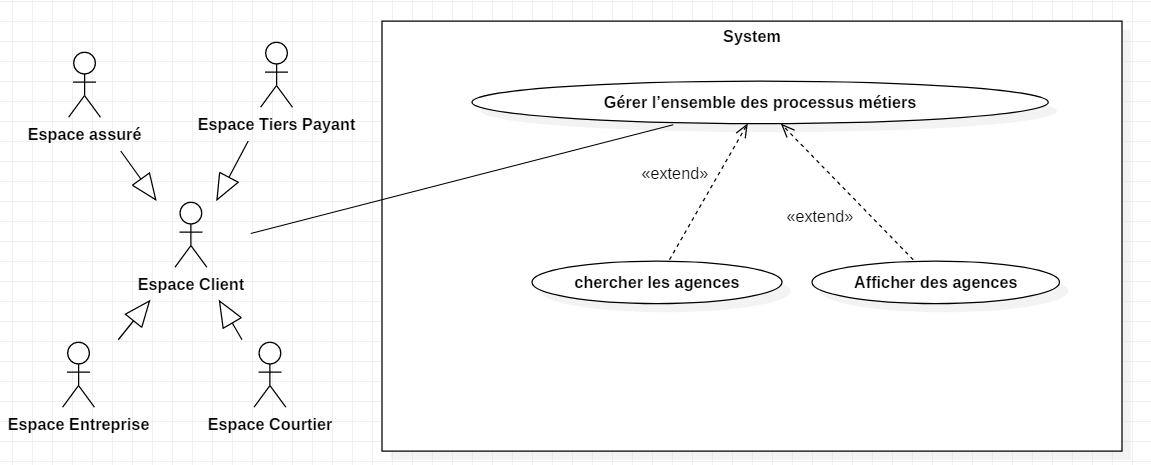
\includegraphics[width=1\columnwidth]{images/use2.PNG}
\caption{Diagramme de cas d'utilisation gestion des agences}
\label{fig:Diagramme de cas d'utilisation sprint 1}
\end{figure}

\subsection{Diagramme de séquence système}
Les diagrammes séquence système représentent l’enchaînement dynamique d’un cas d’utilisation: Gestion des agences
\begin{figure}[H]
\centering
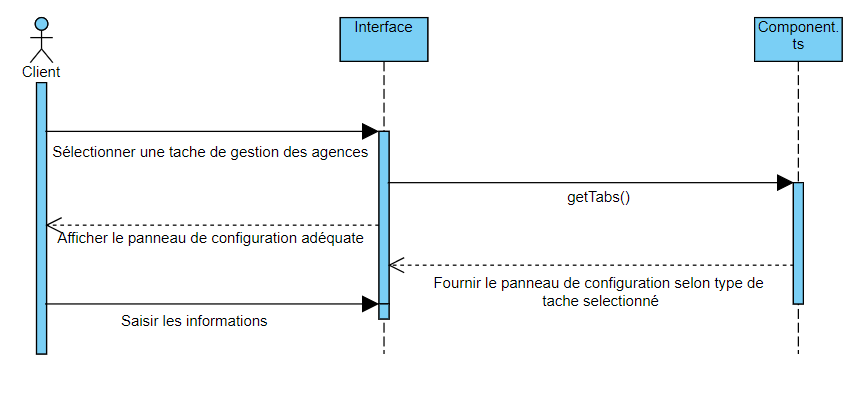
\includegraphics[width=1\columnwidth]{images/seq.PNG}
\caption{Diagramme de séquences de gestion des agences de l'assurance}
\label{fig:Diagramme de cas d'utilisation sprint 1}
\end{figure}





\section{Les tests unitaires}
Nous pouvons tester nos applications Angular de toutes pièces en écrivant et en exécutant des fonctions javascript pures. Créer des instances des classes pertinentes, appeler des fonctions et vérifier le résultat réel par rapport au résultat attendu.
En deux mots un test unitaire est un morceau de code qui valide l'unité par:\\
\textbf{L'appeler avec des intrants spécifiques.}\\
\textbf{Vérification de la sortie par rapport à la valeur attendue.}\\
Mais puisque testing est une activité si courante avec javascript, il existe un certain nombre de bibliothèques de tests et de frameworks que nous pouvons utiliser pour réduire le temps nécessaire pour écrire des tests, comme Jasmine, Mocha, QUnit et Karma.
Deux outils et frameworks de ce type qui sont utilisés lors des tests Angular sont Jasmine et Karma et qui sont les plus utilisés.
\section{IHM}
\begin{figure}[H]
\centering
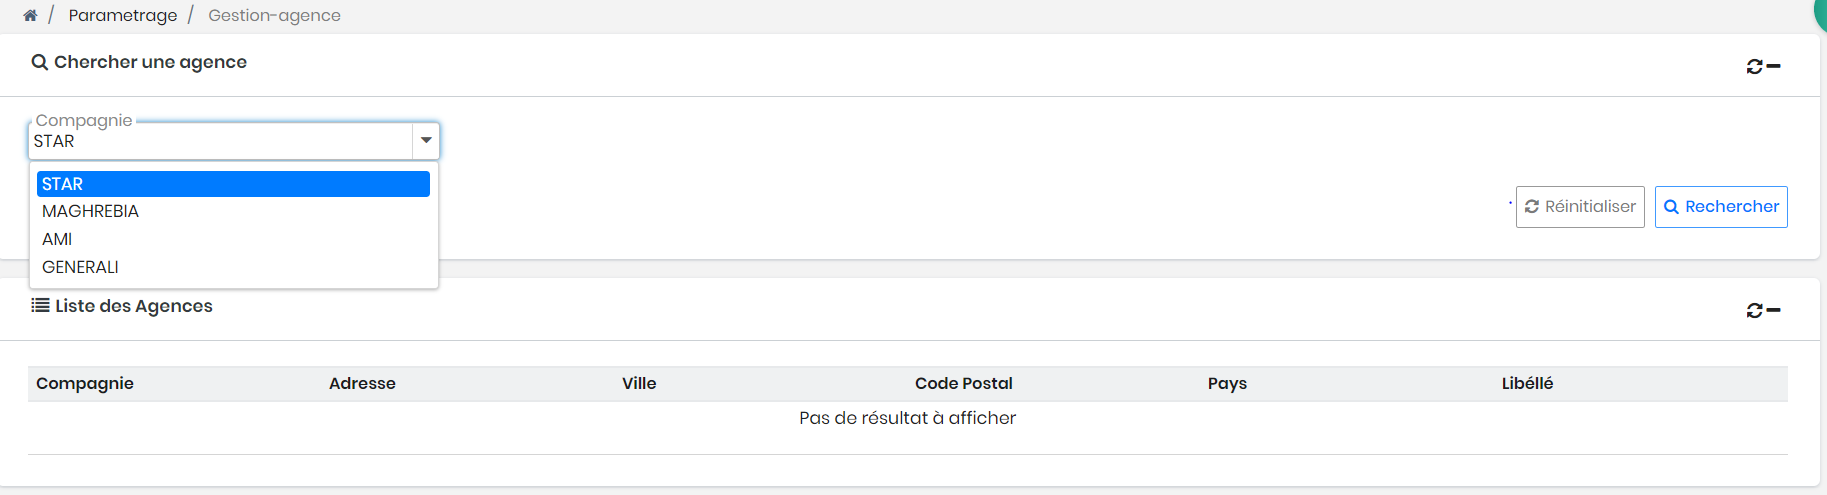
\includegraphics[width=1.05\columnwidth,height=0.45
\columnwidth]{images/interface1.PNG}
\caption{Interfaces de recherche des agences}
\label{fig:Diagramme de cas d'utilisation sprint 1}
\end{figure}





\section*{Conclusion}
Dans ce chapitre nous avons réussi à mettre en place une interface de gestions des agences. En effet, le client peut effectuer la recherche des agences en introduisant juste leur nom de compagnie.